

\bta{2018}



\section{Use of English}

\noindent
\textbf{Directions:}\\
Read the following text. Choose the best word (s) for each numbered blank
and mark A, B, C or D on the ANSWER SHEET. (10 points)



\TiGanSpace

Trust is a tricky business. On the one hand, it's a necessary
condition \cloze many worthwhile things: child care, friendships,
etc. On the other hand, putting your \cloze in the wrong place
often carries a high \cloze.

\cloze , why do we trust at all? Well, because it feels good.
\cloze people place their trust in an individual or an
institution, their brains release oxytocin, a hormone that \cloze
pleasurable feelings and triggers the herding instinct that prompts
humans to \cloze with one another. Scientists have found that
exposure \cloze this hormone puts us in a trusting \cloze
: In a Swiss study, researchers sprayed oxytocin into the noses of half
the subjects; those subjects were ready to lend significantly higher
amounts of money to strangers than were their \cloze who inhaled
something else.

\cloze for us, we also have a sixth sense for dishonesty that
may \cloze us. A Canadian study found that children as young as
14 months can differentiate \cloze a credible person and a
dishonest one. Sixty toddlers were each \cloze to an adult
tester holding a plastic container. The tester would ask, " What's in
here?" before looking into the container, smiling, and exclaiming,
" Wow!" Each subject was then invited to look \cloze. Half of
them found a toy; the other half \cloze the container was
empty---and realized the tester had \cloze them.

Among the children who had not been tricked, the majority were
\cloze to cooperate with the tester in learning a new skill,
demonstrating that they trusted his leadership. \cloze , only
five of the 30 children paired with the " \cloze " tester
participated in a follow-up activity.



\newpage

\begin{enumerate}
	%\renewcommand{\labelenumi}{\arabic{enumi}.}
	% A(\Alph) a(\alph) I(\Roman) i(\roman) 1(\arabic)
	%设定全局标号series=example	%引用全局变量resume=example
	%[topsep=-0.3em,parsep=-0.3em,itemsep=-0.3em,partopsep=-0.3em]
	%可使用leftmargin调整列表环境左边的空白长度 [leftmargin=0em]
	\item

\fourchoices
{from}
{for}
{like}
{on}



\item

\fourchoices
{attention}
{concern}
{faith}
{interest}



\item

\fourchoices
{benefit}
{price}
{debt}
{hope}


\item

\fourchoices
{Again}
{Instead}
{Therefore}
{Then}



\item

\fourchoices
{When}
{Unless}
{Although}
{Until}


\item

\fourchoices
{selects}
{applies}
{produces}
{maintains}



\item

\fourchoices
{connect}
{compete}
{consult}
{compare}



\item

\fourchoices
{by}
{to}
{of}
{at}


\item

\fourchoices
{context}
{circle}
{period}
{mood}



\item

\fourchoices
{counterparts}
{colleagues}
{substitutes}
{supporters}



\item

\fourchoices
{Odd}
{Funny}
{Lucky}
{Ironic}


\item

\fourchoices
{protect}
{delight}
{surprise}
{monitor}


\item

\fourchoices
{over}
{within}
{toward}
{between}


\item

\fourchoices
{added}
{transferred}
{introduced}
{entrusted}



\item

\fourchoices
{out}
{inside}
{back}
{around}


\item

\fourchoices
{proved}
{remembered}
{insisted}
{discovered}


\item

\fourchoices
{fooled}
{mocked}
{betrayed}
{wronged}



\item

\fourchoices
{forced}
{willing}
{hesitant}
{entitled}


\item

\fourchoices
{On the whole}
{As a result}
{For instance}
{In contrast}


\item

\fourchoices
{incapable}
{inflexible}
{unreliable}
{unsuitable}

\end{enumerate}

\vfil

\section{Reading Comprehension}


\noindent
\textbf{Part A}\\
\textbf{Directions:}\\
Read the following four texts. Answer the questions after each text by
choosing A, B, C or
D. Mark your answers on the ANSWER SHEET. (40
points)

\newpage
\subsection{Text 1}


Among the annoying challenges facing the middle class is one that will
probably go unmentioned in the next presidential campaign: What happens
when the robots come for their jobs?

Don't dismiss that possibility entirely. About half of U.S. jobs are
at high risk of being automated, according to a University of Oxford
study, with the middle class disproportionately squeezed. Lower-income
jobs like gardening or day care don't appeal to robots. But many
middle-class occupations---trucking, financial advice, software
engineering---have aroused their interest, or soon will. The rich own
the robots, so they will be fine.

This isn't to be alarmist. Optimists point out that technological
upheaval has benefited workers in the past. The Industrial Revolution
didn't go so well for Luddites whose jobs were displaced by mechanized
looms, but it eventually raised living standards and created more jobs
than it destroyed. Likewise, automation should eventually boost
productivity, stimulate demand by driving down prices, and free workers
from hard, boring work. But in the medium term, middle-class workers
may need a lot of help adjusting.

The first step, as Erik Brynjolfsson and Andrew McAfee argue in
\emph{The Second Machine Age}, should be rethinking education and job
training. Curriculums---from grammar school to college---should evolve
to focus less on memorizing facts and more on creativity and complex
communication. Vocational schools should do a better job of fostering
problem-solving skills and helping students work alongside robots.
Online education can supplement the traditional kind. It could make
extra training and instruction affordable. Professionals trying to
acquire new skills will be able to do so without going into debt.

The challenge of coping with automation underlines the need for the
U.S. to revive its fading business dynamism: Starting new companies must
be made easier. In previous eras of drastic technological change,
entrepreneurs smoothed the transition by dreaming up ways to combine
labor and machines. The best uses of 3 D printers and virtual reality
haven't been invented yet. The U.S. needs the new companies that will
invent them.

Finally, because automation threatens to widen the gap between capital
income and labor income, taxes and the safety net will have to be
rethought. Taxes on low-wage labor need to be cut, and wage subsidies
such as the earned income tax credit should be expanded: This would
boost incomes, encourage work, reward companies for job creation, and
reduce inequality.

Technology will improve society in ways big and small over the next few
years, yet this will be little comfort to those who find their lives and
careers upended by automation. Destroying the machines that are coming
for our jobs would be nuts. But policies to help workers adapt will be
indispensable.

\begin{enumerate}[resume]
	%\renewcommand{\labelenumi}{\arabic{enumi}.}
	% A(\Alph) a(\alph) I(\Roman) i(\roman) 1(\arabic)
	%设定全局标号series=example	%引用全局变量resume=example
	%[topsep=-0.3em,parsep=-0.3em,itemsep=-0.3em,partopsep=-0.3em]
	%可使用leftmargin调整列表环境左边的空白长度 [leftmargin=0em]
	\item
Who will be most threatened by automation?


\fourchoices
{Leading politicians.}
{Low-wage laborers.}
{Robot owners.}
{Middle-class workers.}


\item
Which of the following best represents the author's view?


\fourchoices
{Worries about automation are in fact groundless.}
{Optimists' opinions on new tech find little support.}
{Issues arising from automation need to be tackled.}
{Negative consequences of new tech can be avoided.}


\item
Education in the age of automation should put more emphasis on \lineread.


\fourchoices
{creative potential}
{job-hunting skills}
{individual needs}
{cooperative spirit}


\item
The author suggests that tax policies be aimed at \lineread.


\fourchoices
{encouraging the development of automation}
{increasing the return on capital investment}
{easing the hostility between rich and poor}
{preventing the income gap from widening}

\item
In this text, the author presents a problem with \lineread.


\fourchoices
{opposing views on it}
{possible solutions to it}
{its alarming impacts}
{its major variations}

\end{enumerate}


\newpage
\subsection{Text 2}


A new survey by Harvard University finds more than two-thirds of young
Americans disapprove of President Trump's use of Twitter. The
implication is that Millennials prefer news from the White House to be
filtered through other sources, not a president's social media platform.

Most Americans rely on social media to check daily headlines. Yet as
distrust has risen toward all media, people may be starting to
\uline{beef up} their media literacy skills. Such a trend is badly
needed. During the 2016 presidential campaign, nearly a quarter of web
content shared by Twitter users in the politically critical state of
Michigan was fake news, according to the University of Oxford. And a
survey conducted for BuzzFeed News found 44 percent of Facebook users
rarely or never trust news from the media giant.

Young people who are digital natives are indeed becoming more skillful
at separating fact from fiction in cyberspace. A Knight Foundation
focus-group survey of young people between ages 14 and 24 found they use
``distributed trust'' to verify stories. They cross-check sources and
prefer news from different perspectives---especially those that are open
about any bias. ``Many young people assume a great deal of personal
responsibility for educating themselves and actively seeking out
opposing viewpoints,'' the survey concluded.

Such active research can have another effect. A 2014 survey conducted
in Australia, Britain, and the United States by the University of
Wisconsin-Madison found that young people's reliance on social media led
to greater political engagement.

Social media allows users to experience news events more intimately and
immediately while also permitting them to re-share news as a projection
of their values and interests. This forces users to be more conscious
of their role in passing along information. A survey by Barna research
group found the top reason given by Americans for the fake news
phenomenon is ``reader error,'' more so than made-up stories or factual
mistakes in reporting. About a third say the problem of fake news lies
in ``misinterpretation or exaggeration of actual news'' via social
media. In other words, the choice to share news on social media may be
the heart of the issue. ``This indicates there is a real personal
responsibility in counteracting this problem,'' says Roxanne Stone,
editor in chief at Barna Group.

So when young people are critical of an over-tweeting president, they
reveal a mental discipline in thinking skills---and in their choices on
when to share on social media.


\begin{enumerate}[resume]
	%\renewcommand{\labelenumi}{\arabic{enumi}.}
	% A(\Alph) a(\alph) I(\Roman) i(\roman) 1(\arabic)
	%设定全局标号series=example	%引用全局变量resume=example
	%[topsep=-0.3em,parsep=-0.3em,itemsep=-0.3em,partopsep=-0.3em]
	%可使用leftmargin调整列表环境左边的空白长度 [leftmargin=0em]
	\item
According to Paragraphs 1 and 2, many young Americans cast doubt on \lineread.


\fourchoices
{the justification of the news-filtering practice}
{people's preference for social media platforms}
{the administration's ability to handle information}
{social media as a reliable source of news}


\item
The phrase " beef up'' (Para. 2) is closest in meaning to \lineread.


\fourchoices
{sharpen}
{define}
{boast}
{share}



\item
According to the Knight Foundation survey, young people \lineread.


\fourchoices
{tend to voice their opinions in cyberspace}
{verify news by referring to diverse sources}
{have a strong sense of social responsibility}
{like to exchange views on ``distributed trust''}


\item
The Barna survey found that a main cause for the fake news problem
is \lineread.


\fourchoices
{readers' outdated values}
{journalists' biased reporting}
{readers' misinterpretation}
{journalists' made-up stories}


\item
Which of the following would be the best title for the text?


\fourchoices
{A Rise in Critical Skills for Sharing News Online}
{A Counteraction Against the Over-tweeting Trend}
{The Accumulation of Mutual Trust on Social Media}
{The Platforms for Projection of Personal Interests}


\end{enumerate}


\newpage
\subsection{Text 3}


Any fair-minded assessment of the dangers of the deal between Britain's
National Health Service (NHS) and DeepMind must start by acknowledging
that both sides mean well. DeepMind is one of the leading artificial
intelligence (AI) companies in the world. The potential of this work
applied to healthcare is very great, but it could also lead to further
concentration of power in the tech giants. It is against that
background that the information commissioner, Elizabeth Denham, has
issued her damning verdict against the Royal Free Hospital trust under
the NHS, which handed over to DeepMind the records of 1.6 million
patients in 2015 on the basis of a vague agreement which took far too
little account of the patients' rights and their expectations of
privacy.

DeepMind has almost apologized. The NHS trust has mended its ways.
Further arrangements---and there may be many---between the NHS and
DeepMind will be carefully scrutinised to ensure that all necessary
permissions have been asked of patients and all unnecessary data has
been cleaned. There are lessons about informed patient consent to
learn. But privacy is not the only angle in this case and not even the
most important. Ms Denham chose to concentrate the blame on the NHS
trust, since under existing law it ``controlled'' the data and DeepMind
merely ``processed'' it. But this distinction misses the point that it
is processing and aggregation, not the mere possession of bits, that
gives the data value.

The great question is who should benefit from the analysis of all the
data that our lives now generate. Privacy law builds on the concept of
damage to an individual from identifiable knowledge about them. That
misses the way the surveillance economy works. The data of an
individual there gains its value only when it is compared with the data
of countless millions more.

The use of privacy law to curb the tech giants in this instance feels
slightly maladapted. This practice does not address the real worry. It
is not enough to say that the algorithms DeepMind develops will benefit
patients and save lives. What matters is that they will belong to a
private monopoly which developed them using public resources. If
software promises to save lives on the scale that drugs now can, big
data may be expected to behave as big pharma has done. We are still at
the beginning of this revolution and small choices now may turn out to
have gigantic consequences later. A long struggle will be needed to
avoid a future of digital feudalism. Ms Denham's report is a welcome
start.

\begin{enumerate}[resume]
	%\renewcommand{\labelenumi}{\arabic{enumi}.}
	% A(\Alph) a(\alph) I(\Roman) i(\roman) 1(\arabic)
	%设定全局标号series=example	%引用全局变量resume=example
	%[topsep=-0.3em,parsep=-0.3em,itemsep=-0.3em,partopsep=-0.3em]
	%可使用leftmargin调整列表环境左边的空白长度 [leftmargin=0em]
	\item
 What is true of the agreement between the NHS and DeepMind?


\fourchoices
{It caused conflicts among tech giants.}
{It failed to pay due attention to patients' rights.}
{It fell short of the latter's expectations.}
{It put both sides into a dangerous situation.}





\item
The NHS trust responded to Denham's verdict with \lineread.


\fourchoices
{empty promises}
{tough resistance}
{necessary adjustments}
{sincere apologies}



\item
The author argues in Paragraph 2 that \lineread.


\fourchoices
{privacy protection must be secured at all costs}
{leaking patients' data is worse than selling it}
{making profits from patients' data is illegal}
{the value of data comes from the processing of it}





\item
 According to the last paragraph, the real worry arising from this
deal is \lineread.


\fourchoices
{the vicious rivalry among big pharmas}
{the ineffective enforcement of privacy law}
{the uncontrolled use of new software}
{the monopoly of big data by tech giants}


\item
The author's attitude toward the application of AI to healthcare is \lineread.


\fourchoices
{ambiguous}
{cautious}
{appreciative}
{contemptuous}

	
\end{enumerate}


\newpage
\subsection{Text 4}


The U.S. Postal Service (USPS) continues to bleed red ink. It reported
a net loss of \$5.6 billion for fiscal 2016, the 10th
straight year its expenses have exceeded revenue. Meanwhile, it has
more than \$120 billion in unfunded liabilities, mostly for employee
health and retirement costs. There are many reasons this formerly
stable federal institution finds itself on the verge of bankruptcy.
Fundamentally, the USPS is in a historic squeeze between technological
change that has permanently decreased demand for its bread-and-butter
product, first-class mail, and a regulatory structure that denies
management the flexibility to adjust its operations to the new reality.

And interest groups ranging from postal unions to greeting-card makers
exert self-interested pressure on the USPS's ultimate
overseer---Congress---insisting that whatever else happens to the Postal
Service, aspects of the status quo they depend on get protected. This
is why repeated attempts at reform legislation have failed in recent
years, leaving the Postal Service unable to pay its bills except by
deferring vital modernization.

Now comes word that everyone involved---Democrats, Republicans, the
Postal Service, the unions and the system's heaviest users---has finally
agreed on a plan to fix the system. Legislation is moving through the
House that would save USPS an estimated \$28.6 billion over five years,
which could help pay for new vehicles, among other survival measures.
Most of the money would come from a penny-per-letter permanent rate
increase and from shifting postal retirees into Medicare. The latter
step would largely offset the financial burden of annually pre-funding
retiree health care, thus addressing a long-standing complaint by the
USPS and its unions.

If it clears the House, this measure would still have to get through
the Senate---where someone is bound to point out that it amounts to the
bare, bare minimum necessary to keep the Postal Service afloat, not
comprehensive reform. There's no change to collective bargaining at the
USPS, a major omission considering that personnel accounts for 80
percent of the agency's costs. Also missing is any discussion of
eliminating Saturday letter delivery. That common-sense change enjoys
wide public support and would save the USPS \$2 billion per year. But
postal special-interest groups seem to have killed it, at least in the
House. The emerging consensus around the bill is a sign that
legislators are getting frightened about a politically embarrassing
short-term collapse at the USPS. It is not, however, a sign that
they're getting serious about transforming the postal system for the
21st century.

\begin{enumerate}[resume]
	%\renewcommand{\labelenumi}{\arabic{enumi}.}
	% A(\Alph) a(\alph) I(\Roman) i(\roman) 1(\arabic)
	%设定全局标号series=example	%引用全局变量resume=example
	%[topsep=-0.3em,parsep=-0.3em,itemsep=-0.3em,partopsep=-0.3em]
	%可使用leftmargin调整列表环境左边的空白长度 [leftmargin=0em]
	\item
The financial problem with the USPS is caused partly by \lineread.


\fourchoices
{its unbalanced budget}
{its rigid management}
{the cost for technical upgrading}
{the withdrawal of bank support}


\item
According to Paragraph 2, the USPS fails to modernize itself due to \lineread.


\fourchoices
{the interference from interest groups}
{the inadequate funding from Congress}
{the shrinking demand for postal service}
{the incompetence of postal unions}



\item
The long-standing complaint by the USPS and its unions can be
addressed by \lineread.


\fourchoices
{removing its burden of retiree health care}
{making more investment in new vehicles}
{adopting a new rate-increase mechanism}
{attracting more first-class mail users}

\item
In the last paragraph, the author seems to view legislators with \lineread.


\fourchoices
{respect}
{tolerance}
{discontent}
{gratitude}


\item
Which of the following would be the best title for the text?


\fourchoices
{The USPS Starts to Miss Its Good Old Days}
{The Postal Service: Keep Away from My Cheese}
{The USPS: Chronic Illness Requires a Quick Cure}
{The Postal Service Needs More than a Band-Aid}

	
\end{enumerate}


\newpage

\noindent
\textbf{Part B}\\
\textbf{Directions:}\\
The following paragraphs are given in a wrong order. For questions
41-45, you are required to reorganize these paragraphs into a coherent
text by choosing from the list A-G and filling them into the numbered
boxes. Paragraphs C and F have been correctly placed. Mark your
answers on the ANSWER SHEET. (10 points)


\begin{listmatch}

\item 
 In December of 1869, Congress appointed a commission to select a site
and prepare plans and cost estimates for a new State Department
Building. The commission was also to consider possible arrangements for
the War and Navy Departments. To the horror of some who expected a Greek
Revival twin of the Treasury Building to be erected on the other side of
the White House, the elaborate French Second Empire style design by
Alfred Mullett was selected, and construction of a building to house all
three departments began in June of 1871.


\item 
Completed in 1875, the State Department's south wing was the first to
be occupied, with its elegant four-story library (completed in 1876),
Diplomatic Reception Room, and Secretary's office decorated with carved
wood, Oriental rugs, and stenciled wall patterns. The Navy Department
moved into the east wing in 1879, where elaborate wall and ceiling
stenciling and marquetry floors decorated the office of the Secretary.


\item 
The State, War, and Navy Building, as it was originally known, housed
the three Executive Branch Departments most intimately associated with
formulating and conducting the nation's foreign policy in the last
quarter of the nineteenth century and the first quarter of the twentieth
century---the period when the United States emerged as an international
power. The building has housed some of the nation's most significant
diplomats and politicians and has been the scene of many historic
events.


\item 
Many of the most celebrated national figures have participated in
historical events that have taken place within the EEOB's granite walls.
Theodore and Franklin D. Roosevelt, William Howard Taft, Dwight D. Eisenhower, Lyndon
B. Johnson, Gerald Ford, and George H. W. Bush all
had offices in this building before becoming President. It has housed 16
Secretaries of the Navy, 21 Secretaries of War, and 24 Secretaries of
State. Winston Churchill once walked its corridors and Japanese
emissaries met here with Secretary of State Cordell Hull after the
bombing of Pearl Harbor.


\item 
The Eisenhower Executive Office Building (EEOB) commands a unique
position in both the national history and the architectural heritage of
the United States. Designed by Supervising Architect of the Treasury,
Alfred B. Mullett, it was built from 1871 to 1888 to house the growing
staffs of the State, War, and Navy Departments, and is considered one of
the best examples of French Second Empire architecture in the country.


\item 
Construction took 17 years as the building slowly rose wing by wing.
When the EEOB was finished, it was the largest office building in
Washington, with nearly 2 miles of black and white tiled corridors.
Almost all of the interior detail is of cast iron or plaster; the use of
wood was minimized to insure fire safety. Eight monumental curving
staircases of granite with over 4,000 individually cast bronze balusters
are capped by four skylight domes and two stained glass rotundas.


\item 
The history of the EEOB began long before its foundations were laid.
The first executive offices were constructed between 1799 and 1820. A
series of fires (including those set by the British in 1814) and
overcrowded conditions led to the construction of the existing Treasury
Building. In 1866, the construction of the North Wing of the Treasury
Building necessitated the demolition of the State Department building.

\end{listmatch}

\[ 
\begin{tabular}{|c|c|}
	\hline
	41. &  \hspace{1.5em} \\
	\hline
\end{tabular}
\rightarrow
\begin{tabular}{|c|}
	\hline
	C \\
	\hline
\end{tabular}
\rightarrow
\begin{tabular}{|c|c|}
	\hline
	42. &  \hspace{1.5em} \\
	\hline
\end{tabular}
\rightarrow
\begin{tabular}{|c|c|}
	\hline
	43. &  \hspace{1.5em} \\
	\hline
\end{tabular}
\rightarrow
\begin{tabular}{|c|}
	\hline
	E \\
	\hline
\end{tabular}
\rightarrow
\begin{tabular}{|c|c|}
	\hline
	44. &  \hspace{1.5em} \\
	\hline
\end{tabular}
\rightarrow
\begin{tabular}{|c|c|}
	\hline
	45. &  \hspace{1.5em} \\
	\hline
\end{tabular}
\]


\phantom{ \linefill \linefill \linefill \linefill \linefill}


\newpage

\noindent
\textbf{Part C}\\
\textbf{Directions:}\\
Read the following text carefully and then translate the underlined
segments into Chinese. Write your answers on the ANSWER SHEET. (10
points)


\TiGanSpace

Shakespeare's lifetime was coincident with a period of extraordinary
activity and achievement in the drama. \transnum \uline{By the date of
	his birth Europe was witnessing the passing of the religious drama, and
	the creation of new forms under the incentive of classical tragedy and
	comedy.} These new forms were at first mainly written by scholars and
performed by amateurs, but in England, as everywhere else in western
Europe, the growth of a class of professional actors was threatening to
make the drama popular, whether it should be new or old, classical or
medieval, literary or farcical. Court, school, organizations of
amateurs, and the traveling actors were all rivals in supplying a
widespread desire for dramatic entertainment; and \transnum \uline{no boy
	who went to a grammar school could be ignorant that the drama was a form
	of literature which gave glory to Greece and Rome and might yet bring
	honor to England.}

When Shakespeare was twelve years old the first public playhouse was
built in London. For a time literature showed no interest in this public
stage. Plays aiming at literary distinction were written for schools or
court, or for the choir boys of St. Paul's and the royal chapel, who,
however, gave plays in public as well as at court. \transnum \uline{But
	the professional companies prospered in their permanent theaters, and
	university men with literary ambitions were quick to turn to these
	theaters as offering a means of livelihood.} By the time that
Shakespeare was twenty-five, Lyly, Peele, and Greene had made comedies
that were at once popular and literary; Kyd had written a tragedy that
crowded the pit; and Marlowe had brought poetry and genius to triumph on
the common stage---where they had played no part since the death of
Euripides. \transnum \uline{A native literary drama had been created, its
	alliance with the public playhouses established, and at least some of
	its great traditions had been begun.}

The development of the Elizabethan drama for the next twenty-five years
is of exceptional interest to students of literary history, for in this
brief period we may trace the beginning, growth, blossoming, and decay
of many kinds of plays, and of many great careers. We are amazed today
at the mere number of plays produced, as well as by the number of
dramatists writing at the same time for this London of two hundred
thousand inhabitants. \transnum \uline{To realize how great was the
	dramatic activity, we must remember further that hosts of plays have
	been lost, and that probably there is no author of note whose entire
	work has survived.}


\newpage
\section{Writing}


\noindent
\textbf{Part A}\\
51. \textbf{Directions:}

Write an email to all international experts on campus, inviting them to
attend the graduation ceremony. In your email, you should include the
time, place and other relevant information about the ceremony.

You should write about 100 words on the ANSEWER SHEET

\textbf{Do not} use your own name at the end of the email. Use ``Li
Ming'' instead. (10 points)

\vspace{2em}

\noindent
\textbf{Part B}\\
52. \textbf{Directions:}

Write an essay of 160-200 words based on the picture below. In your
essay, you should
\begin{listwrite}
	%\renewcommand{\labelenumi}{\arabic{enumi}.}
	% A(\Alph) a(\alph) I(\Roman) i(\roman) 1(\arabic)
	%设定全局标号series=example	%引用全局变量resume=example
	%[topsep=-0.3em,parsep=-0.3em,itemsep=-0.3em,partopsep=-0.3em]
	%可使用leftmargin调整列表环境左边的空白长度 [leftmargin=0em]
	\item
describe the picture briefly,

\item 
 interpret the meaning, and

\item 
 give your comments.
\end{listwrite}


Write your answer on the ANSWER SHEET. (20 points)


\begin{figure}[h!]
	\centering
	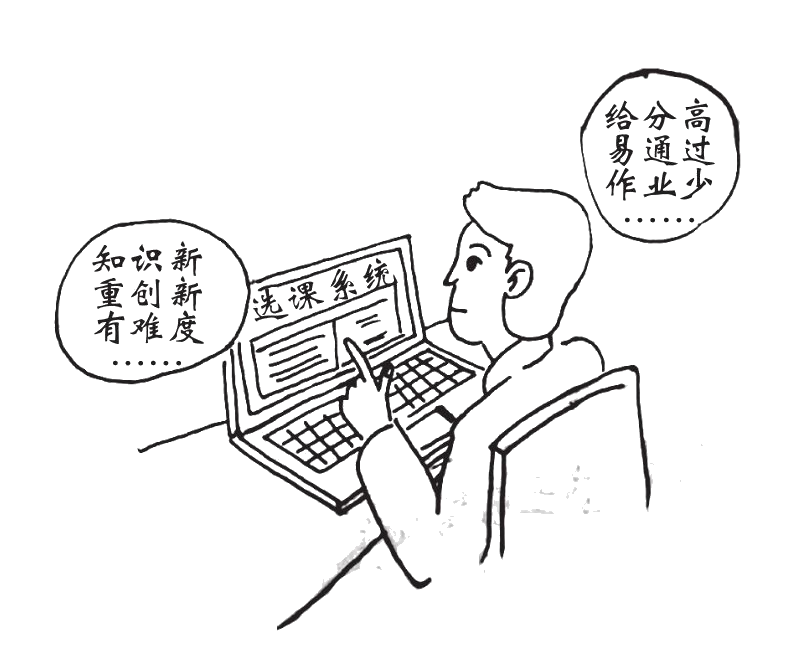
\includegraphics[width=0.53\linewidth]{picture/2018.png}
	\caption*{选课进行时}
\end{figure}



\checkpagenumber